\begin{Answer}{1}
	\begin{enumerate}[a),leftmargin=*]
		\i \hspace*{80pt}
		\begin{tikzpicture}
			\draw (-4,0) -- (4,0);
			\filldraw[black] (-2,0) circle[radius = 2pt] node[above] {$A$};
			\filldraw[black] (2,0) circle[radius = 2pt] node[above] {$B$};
		\end{tikzpicture}
		\i \hspace*{120pt}
		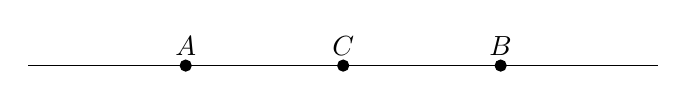
\begin{tikzpicture}
			\draw (-4,0) -- (4,0);
			\filldraw[black] (-2,0) circle[radius = 2pt] node[above] {$A$};
			\filldraw[black] (0,0) circle[radius = 2pt] node[above] {$C$};
			\filldraw[black] (2,0) circle[radius = 2pt] node[above] {$B$};
		\end{tikzpicture}
		\i \hspace*{120pt}
		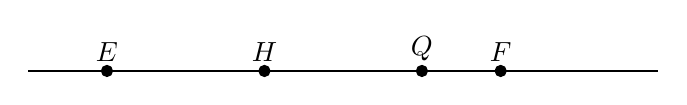
\begin{tikzpicture}
			\draw (-4,0) -- (4,0);
			\filldraw[black] (-3,0) circle[radius = 2pt] node[above] {$E$};
			\filldraw[black] (-1,0) circle[radius = 2pt] node[above] {$H$};
			\filldraw[black] (1,0) circle[radius = 2pt] node[above] {$Q$};
			\filldraw[black] (2,0) circle[radius = 2pt] node[above] {$F$};
		\end{tikzpicture}
		\i \hspace*{170pt}
		\begin{tikzpicture}
			\draw  (-2.,2.)-- (2.,0.);
			\draw  (-1.7,0.02)-- (1.94,1.68);
			\draw [fill=uuuuuu] (0.21413793103448267,0.8929310344827588) circle (2.0pt);
			\draw[color=uuuuuu] (0.36,1.23) node {$P$};
			\draw [fill=xdxdff] (-1.016,1.508) circle (2.0pt);
			\draw[color=xdxdff] (-0.88,1.87) node {$E$};
			\draw [fill=xdxdff] (-0.9032809336965487,0.38333891485267285) circle (2.0pt);
			\draw[color=xdxdff] (-0.76,0.75) node {$M$};
			\draw [fill=xdxdff] (1.2051408292304997,1.3448719166270962) circle (2.0pt);
			\draw[color=xdxdff] (1.34,1.71) node {$N$};
		\end{tikzpicture}
	\i \hspace*{120pt}
	\begin{tikzpicture}
		\draw (-4,0) -- (4,0) (0,-0.1) -- (0, 0.1);
		\filldraw[black] (1,0) circle[radius = 2pt] node[above] {$A$};
		\filldraw[black] (3,0) circle[radius = 2pt] node[above] {$B$};
		\draw (-4,0) node [above] {$y$};
		\draw (4,0) node [above] {$x$};
	\end{tikzpicture}
	\end{enumerate}
	
\end{Answer}
\begin{Answer}{2}
		\begin{enumerate}[a),leftmargin=*]
			\i \begin{align*}
				N& \quad\boxed{\notin} \quad n && B \quad\boxed{\in} \quad m\\
				N& \quad\boxed{\in} \quad p && A \quad\boxed{\notin} \quad q\\
				A& \quad\boxed{\in} \quad n && C \quad\boxed{\in} \quad q
			\end{align*}
			\i Bộ ba điểm thẳng hàng:  $M,A,B$.
		\end{enumerate}
	
\end{Answer}
\begin{Answer}{3}
		\begin{enumerate}[--,leftmargin=*]
			\i Hình ảnh về 2 đường thẳng song song: 2 mép bàn, các đường dây điện, song sắt, đường ray tàu hoả, vạch kẻ đường, \ldots
			\begin{center}
				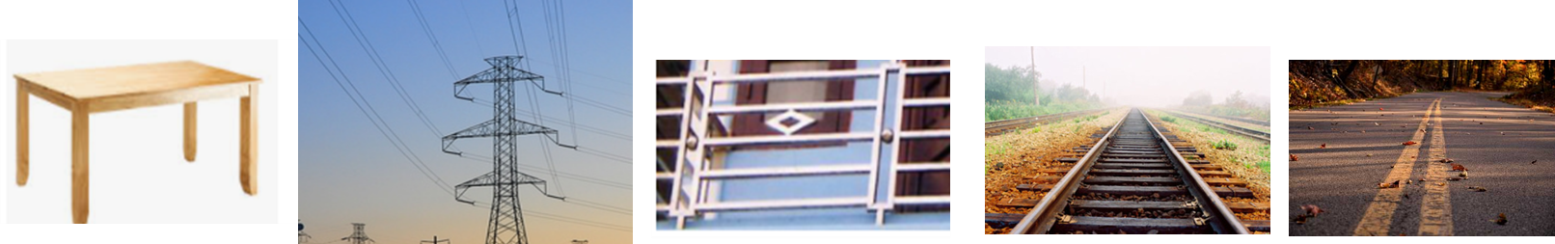
\includegraphics[width=0.75\linewidth]{image029}
			\end{center}
		\i Hình ảnh về 2 đường thẳng cắt nhau: Cái kéo, 2 mép tường, Tia laser, các con đường giao\linebreak thông, \ldots
		\begin{center}
			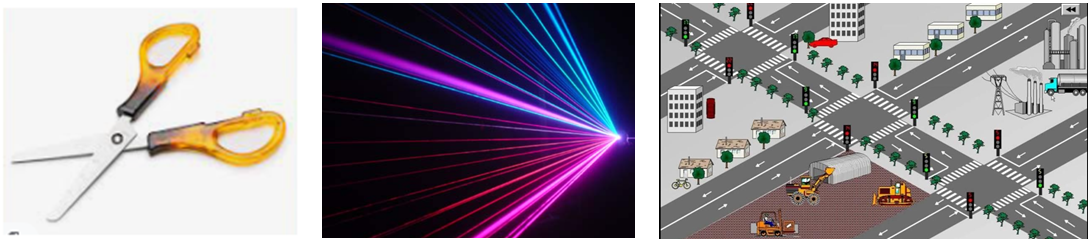
\includegraphics[width=0.75\linewidth]{image030}
		\end{center}
		\end{enumerate}
	
\end{Answer}
\begin{Answer}{4}
		\begin{enumerate}[a),leftmargin=*]
			\i Đường thẳng  $a$ đi qua $M$ và không đi qua $N$.
			\i Đường thẳng $b$ đi qua $Q$  và không đi qua $M$.
			\i Đường thẳng $c$ đi qua cả hai điểm $M,N$
		\end{enumerate}
	
\end{Answer}
\begin{Answer}{5}
	\begin{tabular}{p{0.5\textwidth} p{0.5\textwidth}}
		a)  & b) \\
		\begin{tikzpicture}
			\draw (0,0) -- (4,0) (0,1) -- (4, 1) (0,2) -- (4,2);
			\draw (4,0) node [right] {$c$};
			\draw (4,1) node [right] {$b$};
			\draw (4,2) node [right] {$a$};
		\end{tikzpicture}& 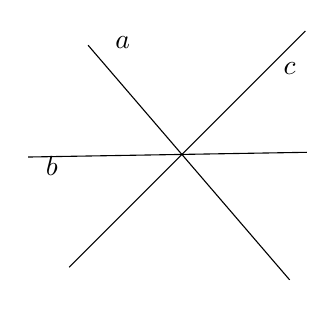
\begin{tikzpicture}
		\draw (0.6,2.88)-- (-2.4,-0.12);
		\draw (0.4,-0.28)-- (-2.16,2.7);
		\draw (-2.92,1.28)-- (0.62,1.34);
		\draw[color=black] (0.4,2.41) node {$c$};
		\draw[color=black] (-1.72,2.73) node {$a$};
		\draw[color=black] (-2.62,1.17) node {$b$};
	\end{tikzpicture} \\
	 c) & d) \\
	 \begin{tikzpicture}
	\draw  (-4.,2.)-- (1.,2.);
	\draw  (-4.,1.)-- (1.,1.);
	\draw  (0.,3.)-- (-3.,0.);
	\draw[color=black] (0.16,1.87) node {$b$};
	\draw[color=black] (0.06,0.87) node {$a$};
	\draw[color=black] (-0.54,2.91) node {$c$};
	\draw [fill=uuuuuu] (-1.,2.) circle (2.0pt);
	\draw [fill=uuuuuu] (-2.,1.) circle (2.0pt);
\end{tikzpicture} & 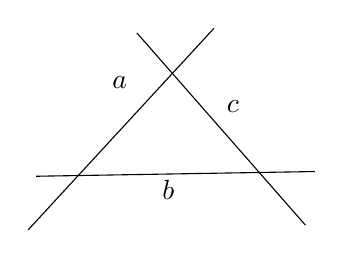
\begin{tikzpicture}
\draw (-0.2,2.64)-- (-2.56,0.08);
\draw (0.96,0.14)-- (-1.18,2.58);
\draw (-2.46,0.76)-- (1.08,0.82);
\draw[color=black] (0.04,1.65) node {$c$};
\draw[color=black] (-1.4,1.95) node {$a$};
\draw[color=black] (-0.78,0.59) node {$b$};
\end{tikzpicture}
	\end{tabular}
	
\end{Answer}
\begin{Answer}{6}
		\begin{tabular}{p{0.5\textwidth} p{0.5\textwidth}}
			a) & b) \\
			\begin{tikzpicture}
				\draw  (-4.,2.)-- (1.,2.);
				\draw  (-3.5,1.14)-- (0.56,2.88);
				\draw[color=black] (-2.76,1.23) node {$x$};
				\draw [fill=uuuuuu] (-1.4933333333333332,2.) circle (2.0pt);
				\draw[color=uuuuuu] (-1.36,2.33) node {$A$};
				\draw [fill=xdxdff] (-3.02,2.) circle (2.0pt);
				\draw[color=xdxdff] (-2.88,2.37) node {$M$};
				\draw [fill=xdxdff] (-0.08,2.) circle (2.0pt);
				\draw[color=xdxdff] (0.06,2.37) node {$N$};
				\draw [fill=xdxdff] (0.11344827586206918,2.6886206896551723) circle (2.0pt);
				\draw[color=xdxdff] (0.26,3.05) node {$P$};
			\end{tikzpicture}&
			\begin{tikzpicture}
				\draw  (-4.,2.)-- (1.,2.);
				\draw  (-2.32,1.)-- (1.74,2.74);
				\draw[color=black] (-1.58,1.09) node {$y$};
				\draw [fill=uuuuuu] (0.013333333333332476,2.) circle (2.0pt);
				\draw[color=uuuuuu] (0.16,2.33) node {$B$};
				\draw [fill=xdxdff] (-3.02,2.) circle (2.0pt);
				\draw[color=xdxdff] (-2.88,2.37) node {$M$};
				\draw [fill=xdxdff] (-1.34,2.) circle (2.0pt);
				\draw[color=xdxdff] (-1.2,2.37) node {$N$};
				\draw [fill=xdxdff] (1.2934482758620685,2.5486206896551726) circle (2.0pt);
				\draw[color=xdxdff] (1.44,2.91) node {$P$};
			\end{tikzpicture}\\
			\multicolumn{2}{l}{c)}\\
			\multicolumn{2}{l}{\begin{tikzpicture}
				\draw  (-4.,2.)-- (1.,2.);
				\draw  (-3.46,2.9)-- (-1.7,0.86);
				\draw [fill=xdxdff] (-0.88,2.) circle (2.0pt);
				\draw[color=xdxdff] (-0.74,2.37) node {$M$};
				\draw [fill=xdxdff] (0.38,2.) circle (2.0pt);
				\draw[color=xdxdff] (0.52,2.37) node {$N$};
				\draw[color=black] (-3.04,2.95) node {$z$};
				\draw [fill=uuuuuu] (-2.683529411764706,2.) circle (2.0pt);
				\draw[color=uuuuuu] (-2.54,2.33) node {$C$};
				\draw [fill=xdxdff] (-2.1179854529424738,1.344483138637867) circle (2.0pt);
				\draw[color=xdxdff] (-1.98,1.71) node {$P$};
			\end{tikzpicture}}
		\end{tabular}
	
\end{Answer}
\begin{Answer}{7}
		Bài 14. Có 6 đoạn thẳng có mút là 2 trong 4 điểm $A,B,C,D$:
		Đoạn thẳng $AB$, $AC$, $AD$, $BC$, $BD$, $CD$.
	
\end{Answer}
\begin{Answer}{8}
		\begin{enumerate}[a),leftmargin=*]
			\i Có tất cả 8 tia: $Ax,Ay,Bx,By,Cx,Cy,Dx,Dy$.
			\i Điểm $B$ nằm trên tia $Ax,Bx,By$.\\
			Tia đối của tia $Ay$ là tia $Ax$.\\
			Tia đối của tia $Ax$ là tia $Ay$.\\
			Tia đối của tia $Bx$ là tia $Bx$.\\
			Tia đối của tia $By$là tia $Bx$.\\
			\i Hai tia $AC$ và tia $CA$ không là hai tia đối nhau
		\end{enumerate}
	
\end{Answer}
\begin{Answer}{9}
		Ta có thể vẽ như sau:
		\begin{center}
			\begin{tikzpicture}
				\draw  (-1.92,4.04)-- (-3.78,1.88);
				\draw  (-3.78,1.88)-- (0.36,1.84);
				\draw  (0.36,1.84)-- (-1.92,4.04);
				\draw  (-3.78,1.88)-- (-0.8624928275422378,3.0195983423653177);
				\draw  (0.36,1.84)-- (-2.8289853788214443,2.9844040762073547);
				\draw  (-1.92,4.04)-- (-1.8201829510185985,1.861064569575059);
		
					\draw [fill=ududff] (-1.92,4.04) circle (2.0pt);
					\draw[color=ududff] (-1.78,4.41) node {$A$};
					\draw [fill=ududff] (-3.78,1.88) circle (2.0pt);
					\draw[color=ududff] (-4.14,1.77) node {$B$};
					\draw [fill=ududff] (0.36,1.84) circle (2.0pt);
					\draw[color=ududff] (0.66,1.91) node {$C$};
					\draw [fill=xdxdff] (-0.8624928275422378,3.0195983423653177) circle (2.0pt);
					\draw[color=xdxdff] (-0.62,3.41) node {$M$};
					\draw [fill=xdxdff] (-2.8289853788214443,2.9844040762073547) circle (2.0pt);
					\draw[color=xdxdff] (-3.26,3.29) node {$N$};
					\draw [fill=xdxdff] (-1.8201829510185985,1.861064569575059) circle (2.0pt);
					\draw[color=xdxdff] (-1.56,1.59) node {$P$};
					\draw [fill=uuuuuu] (-1.8510505349070308,2.6334609113144305) circle (2.0pt);
					\draw[color=uuuuuu] (-1.72,2.97) node {$G$};
		\end{tikzpicture}
		\end{center}
	
\end{Answer}
\begin{Answer}{10}
	Có 10 điểm là giao điểm của đúng 2 đường: $A,B,C,D,E,M,N,O,P,Q.$
	
\end{Answer}
\begin{Answer}{11}
		Do cứ 2 điểm thì tạo thành 1 đường thẳng và không có 3 điểm nào thẳng hàng nên 2022 điểm sẽ nối được với 2021 điểm và mỗi đường thẳng sẽ bị trùng nên ta có:
		
		Số đường thẳng được tạo thành là: $\dfrac{2022.2021}{2}=2043231$ (đường thẳng)
		
		Vậy tạo thành được 2043231 đường thẳng khác nhau có đầu mút là 2 trong 2022 điểm đã cho.
	
\end{Answer}
\begin{Answer}{12}
		Bài 19. Giả sử 1998 điểm phân biệt không có 3 điểm nào thẳng hàng, khi đó:
		
		Số đường thẳng được tạo thành là: $\dfrac{1998.(1998-1)}{2}=1995003$(đường thẳng)
		
		5 điểm thẳng hàng tạo thành 1 đường thẳng.
		
		5 điểm không thẳng hàng tạo thành $\dfrac{5.4}{2}=10$ (đường thẳng)
		
		Số đường thẳng bị giảm đi là: $10-1=9$ (đường thẳng)
		
		Vậy có tất cả: $1995003-9=1994994$ (đường thẳng)
	
\end{Answer}
\begin{Answer}{13}
		Bài 20. Do cứ 2 điểm thì tạo thành 1 đường thẳng và không có 3 đường thẳng nào đồng quy nên cứ mỗi đường thẳng sẽ giao với $n-1$ đường thẳng và tạo ra $n-1$ giao điểm
		
		Vậy với $n$ đường thẳng cắt nhau có số giao điểm là: $\dfrac{n(n-1)}{2}$ (do số giao điểm bị trùng)
		
		Theo đề ra: $\dfrac{n(n-1)}{2}=780 \Leftrightarrow n(n-1)=1560$
		
		Do $40\cdot39=1560$ nên $n=40$(đường thẳng).
	
\end{Answer}
\begin{Answer}{14}
		Bài 21. Giả sử 1015 đường cắt nhau trong đó không có 3 đường thẳng nào đồng quy. Khi đó số đường thẳng được tạo thành là:
		\begin{align*}
			\dfrac{1015\cdot1014}{2}=514605 \text{ (đường thẳng)}
		\end{align*}
		15 đường thẳng đồng quy thì có số giao điểm là 1.
		
		15 đường thẳng không đồng quy thì số giao điểm là:
		\begin{align*}
			\dfrac{15\cdot14}{2}=105 \text{ (đường thẳng)}
		\end{align*}
		Số giao điểm bị giảm là: $105-1=104$(đường thẳng)
		
		Vậy với 1015 đường thẳng cắt nhau trong đó có 15 đường đồng quy thì có số giao điểm là: $514605-104=514501$(đường thẳng)
	
\end{Answer}
\begin{Answer}{15}
		Mỗi một thành viên của đội Thái Bình Dương sẽ kết nối với 8 thành viên của đội Đại Tây Dương cần 8 đường dây.
		
		Vậy 5 thành viên của đội Đại Tây Dương kết nối với 8 thành viên của đội Đại Tây Dương cần: $5\cdot8=40$ (đường dây)
	
\end{Answer}
\begin{Answer}{16}
		\begin{tabular}{p{0.33\linewidth} p{0.33\linewidth} p{0.33\linewidth}}
			a) & b) &c)\\
			\begin{tikzpicture}
				\draw  (-1.52,3.34)-- (0.72,1.68);
				\draw  (-1.52,1.7)-- (0.84,3.28);
					\draw [fill=ududff] (-1.52,3.34) circle (2.0pt);
					\draw [fill=ududff] (0.72,1.68) circle (2.0pt);
					\draw [fill=ududff] (-1.52,1.7) circle (2.0pt);
					\draw [fill=ududff] (0.84,3.28) circle (2.0pt);
					\draw [fill=uuuuuu] (-0.3573436326574405,2.4783885849157814) circle (2.0pt);
			\end{tikzpicture}&
		\begin{tikzpicture}
			\draw  (-1.22,4.24)-- (-2.38,2.);
			\draw  (-2.38,2.)-- (1.14,2.02);
			\draw  (1.14,2.02)-- (-1.22,4.24);
			\draw  (-1.22,4.24)-- (-0.820277625334926,2.008862058946961);
			\draw  (-2.38,2.)-- (-0.18976490760144782,3.2708805486759385);
			\draw  (1.14,2.02)-- (-1.7957706814181542,3.128166960020116);
	
				\draw [fill=ududff] (-1.22,4.24) circle (2.0pt);
				\draw [fill=ududff] (-2.38,2.) circle (2.0pt);
				\draw [fill=ududff] (1.14,2.02) circle (2.0pt);
				\draw [fill=xdxdff] (-0.820277625334926,2.008862058946961) circle (2.0pt);
				\draw [fill=xdxdff] (-0.18976490760144782,3.2708805486759385) circle (2.0pt);
				\draw [fill=xdxdff] (-1.7957706814181542,3.128166960020116) circle (2.0pt);
				\draw [fill=uuuuuu] (-0.9657124187758623,2.8206381969906964) circle (2.0pt);
		\end{tikzpicture}&
	\begin{tikzpicture}[scale=0.6]
		\draw  (-4.,5.)-- (0.,5.);
		\draw  (0.,5.)-- (0.,1.);
		\draw  (0.,1.)-- (-4.,1.);
		\draw  (-4.,1.)-- (-4.,5.);
		\draw  (-2.,5.)-- (-2.,1.);
		\draw  (-4.,3.)-- (0.,3.);
		\draw  (-4.,5.)-- (0.,1.);
		\draw  (-4.,1.)-- (0.,5.);
			\draw [fill=ududff] (-4.,5.) circle (2.0pt);
			\draw [fill=ududff] (0.,5.) circle (2.0pt);
			\draw [fill=ududff] (0.,1.) circle (2.0pt);
			\draw [fill=ududff] (-4.,1.) circle (2.0pt);
			\draw [fill=xdxdff] (-2.,5.) circle (2.0pt);
			\draw [fill=xdxdff] (-2.,1.) circle (2.0pt);
			\draw [fill=xdxdff] (-4.,3.) circle (2.0pt);
			\draw [fill=xdxdff] (0.,3.) circle (2.0pt);
			\draw [fill=uuuuuu] (-2.,3.) circle (2.0pt);
	\end{tikzpicture}
		\end{tabular}
	
\end{Answer}
